\section{File Structure}
\label{methodology:file_structure}

The FlatCityBuf format implements a structured binary encoding designed specifically for efficient storage and retrieval of 3D city models in cloud environments. This section details the physical organisation of the file format and its constituent components.

\subsection{Overall Encoding Structure}
\label{methodology:overall_encoding_structure}

FlatCityBuf employs a hybrid encoding approach that combines FlatBuffers serialisation with custom binary formats for indexing structures. The file consists of five sequentially arranged segments:

\begin{itemize}
  \item \textbf{Magic Bytes}: Four-byte identifier ('FCB\\0') for format validation
  \item \textbf{Header Size}: Four-byte unsigned integer specifying the header length
  \item \textbf{Header}: Metadata and schema information encoded using FlatBuffers
  \item \textbf{Index Section}: Combined spatial and attribute indices for efficient data access
  \item \textbf{Features Section}: Serialised city objects with their associated geometry and attributes
\end{itemize}

Figure~\ref{fig:file-structure} illustrates the structural organisation of a FlatCityBuf file, highlighting the spatial relationships between components and their relative positioning.

% \begin{figure}[ht]
%   \centering
%   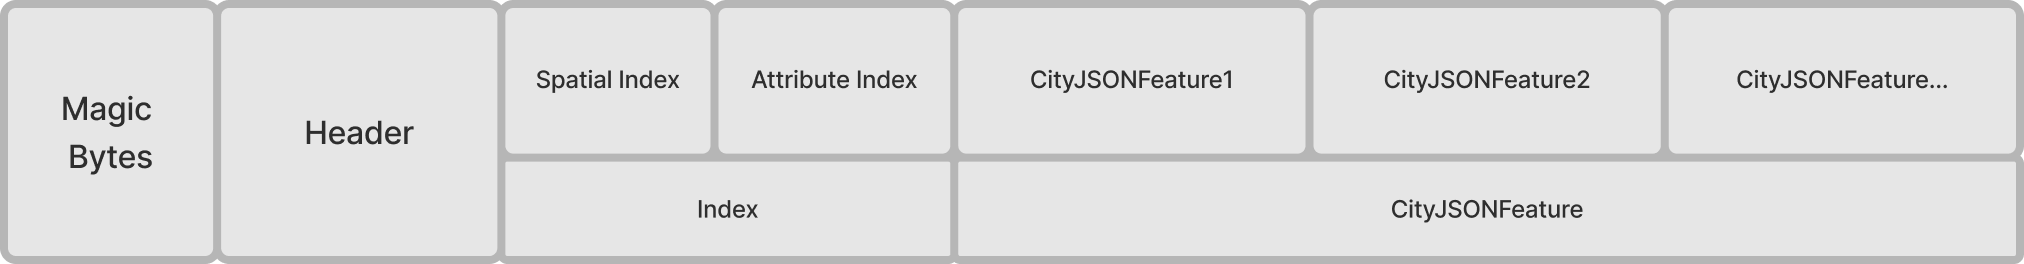
\includegraphics[width=0.8\textwidth]{figures/methodology/file_structure.png}
%   \caption{Physical layout of the FlatCityBuf file format, showing section boundaries and alignment considerations for optimised range requests}
%   \label{fig:file-structure}
% \end{figure}

This sequence-based structure enables incremental file access through HTTP Range Requests—a critical capability for cloud-based applications where minimising data transfer is essential. Each section was designed with explicit consideration for alignment boundaries to optimise I/O operations in both local and networked environments.

\subsection{Magic Bytes and Identification}
\label{methodology:overview:magic_bytes}

The magic bytes section comprises the first four bytes of the file and serves as an immediate identifier for the FlatCityBuf format. This implementation follows established conventions in binary file formats:

\begin{itemize}
  \item The signature consists of the ASCII sequence 'FCB\\0' (0x46 0x43 0x42 0x00)
  \item Applications can validate file integrity and format compatibility by checking these initial bytes
  \item The zero-terminator (\\0) ensures compatibility with null-terminated string operations
\end{itemize}

Following the magic bytes, a 4-byte unsigned integer specifies the size of the header section, enabling applications to locate subsequent sections without parsing the header content.

\subsection{Header Section}
\label{methodology:overview:header_section}

The header section encapsulates metadata essential for interpreting the file contents. Implemented as a FlatBuffers-serialised \texttt{Header} table, it contains:

\begin{itemize}
  \item \textbf{CityJSON Metadata}: Version identifier, coordinate reference system, and transformations
  \item \textbf{Geographical Extent}: Bounding box coordinates defining the spatial coverage
  \item \textbf{Transformation Parameters}: Scale and translation vectors for vertex coordinate interpretation
  \item \textbf{Index Metadata}: Information required to interpret the spatial and attribute indices
  \item \textbf{Schema Information}: Attribute definitions, data types, and extension references
  \item \textbf{Global Appearance}: Materials, textures, and appearance definitions shared across features
\end{itemize}

The header preserves all mandatory elements from the CityJSON specification while adding additional metadata specific to the FlatCityBuf format. This design ensures backward compatibility with existing CityJSON processors while enabling optimised operation for FlatCityBuf-aware applications.

\subsection{Spatial Index Section}
\label{methodology:overview:spatial_index_section}

The spatial index immediately follows the header and implements a Packed Hilbert R-tree structure optimised for two-dimensional spatial queries. This index provides:

\begin{itemize}
  \item \textbf{Hierarchical Spatial Organisation}: Enables logarithmic-time access to features based on spatial location
  \item \textbf{Byte Offset References}: Direct pointers to feature locations within the features section
  \item \textbf{Hilbert Curve Ordering}: Enhances spatial locality for improved query performance
\end{itemize}

The implementation details of the spatial indexing algorithm are fully explained in Section~\ref{methodology:spatial_index}, including node structure, tree construction, and query optimisation techniques.

\subsection{Attribute Index Section}
\label{methodology:overview:attribute_index_section}

Following the spatial index, the attribute index section provides efficient access to features based on their non-spatial properties. Implemented as a series of Static B+trees:

\begin{itemize}
  \item Each indexed attribute has a dedicated B+tree structure
  \item Tree nodes contain key-value pairs linking attribute values to feature offsets
  \item Indices are arranged sequentially based on attribute index order defined in the header
  \item Type-specific serialisation ensures efficient representation of different attribute types
\end{itemize}

The attribute indexing system supports exact-match and range-based queries across multiple attribute types, including numeric, string, and temporal values. Section~\ref{methodology:attribute_index} provides a comprehensive explanation of the B+tree implementation and query algorithms.

\subsection{Features Section}
\label{methodology:overview:features_section}

The features section contains the actual city objects and their associated data, serialised as FlatBuffers tables. Key characteristics include:

\begin{itemize}
  \item Each feature is encoded as a standalone FlatBuffers buffer with length prefix
  \item Features are arranged sequentially with no internal padding or alignment
  \item Features contain multiple city objects sharing common vertices for storage efficiency
  \item Geometry, semantics, attributes, and appearance information are encoded according to the \texttt{CityFeature} schema
\end{itemize}

The internal structure of features follows the CityJSON conceptual model while leveraging FlatBuffers' efficient binary representation. This approach preserves the semantic richness of CityJSON while significantly reducing storage requirements and parse time.

Section~\ref{methodology:feature_encoding} provides detailed information on the feature encoding methodology, including geometry representation, attribute encoding, and semantic model preservation.
